\documentclass[tikz,border=0pt]{standalone}
\usepackage{amsmath}
\usepackage{amssymb}
\usepackage{tikz}
\usetikzlibrary{arrows.meta}

\definecolor{ink}{HTML}{0F172A}
\definecolor{muted}{HTML}{64748B}
\definecolor{gridline}{HTML}{94A3B8}
\definecolor{highlight}{HTML}{CBD5E1}

\begin{document}
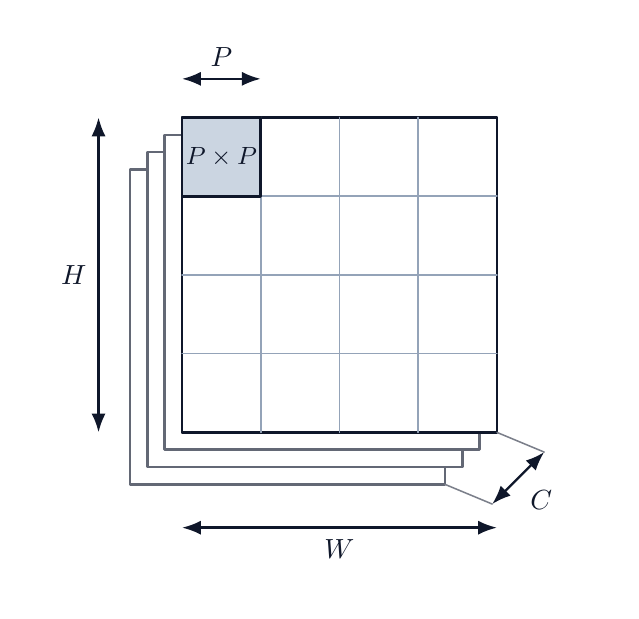
\begin{tikzpicture}[
  font=\sffamily,
  >=Latex,
  line cap=round,
  line join=round
]
  \fill[white] (-1.3,-1.35) rectangle (6.1,5.8);

  % Offset sheets make the channel dimension a stack of images, not a cube.
  \foreach \layer in {0,...,3} {
    \begin{scope}[xshift=\layer*0.22cm,yshift=\layer*0.22cm]
      \draw[ink!65, line width=0.9pt, fill=white] (0,0) rectangle (4,4);
    \end{scope}
  }

  % The front image is partitioned into non-overlapping square patches.
  \begin{scope}[xshift=0.66cm,yshift=0.66cm]
    \draw[ink, line width=1pt, fill=white] (0,0) rectangle (4,4);
    \foreach \column in {1,2,3} {
      \draw[gridline, line width=0.55pt] (\column,0) -- (\column,4);
    }
    \foreach \row in {1,2,3} {
      \draw[gridline, line width=0.55pt] (0,\row) -- (4,\row);
    }
    \fill[highlight] (0,3) rectangle (1,4);
    \draw[ink, line width=1pt] (0,3) rectangle (1,4);
    \node[ink, font=\small] at (0.5,3.5) {$P\times P$};
  \end{scope}

  \draw[ink, <->, line width=0.85pt]
    (-0.4,0.66) -- (-0.4,4.66)
    node[midway, left=3pt, fill=white, inner sep=1pt] {$H$};
  \draw[ink, <->, line width=0.85pt]
    (0.66,-0.55) -- (4.66,-0.55)
    node[midway, below=3pt, fill=white, inner sep=1pt] {$W$};
  \draw[ink, <->, line width=0.85pt]
    (0.66,5.15) -- (1.66,5.15)
    node[midway, above=3pt, fill=white, inner sep=1pt] {$P$};
  % Channel depth: measure the offset from the back sheet to the front sheet.
  \draw[ink!55, line width=0.55pt] (4,0) -- (4.6,-0.25);
  \draw[ink!55, line width=0.55pt] (4.66,0.66) -- (5.26,0.41);
  \draw[ink, <->, line width=0.85pt]
    (4.6,-0.25) -- (5.26,0.41)
    node[midway, below right=3pt, fill=white, inner sep=1pt] {$C$};

\end{tikzpicture}
\end{document}
